\section{Auswertung}
\label{sec:auswertung}

\subsection{Längenbestimmung über Schallgeschwindigkeit in Acryl}

Zunächst wurde die Dicke der Acrylplatte mithilfe einer Schieblehre zu
\begin{equation*}
    D_\text{m} = (10,0 \pm 0,05) \,\unit{\milli\meter}
\end{equation*}
bestimmt.

Um dann die Schallgeschwindigkeit zu ermitteln, wurden die Differenzen zwischen den einzelnen Peaks gemessen.
Wie in \autoref{fig:export1} zu erkennen, wurde das Messfenster so eingestellt, dass vier Impulse zu sehen waren.
Die Differenzen $T_{i,i+1}$ zwischen dem $i$-ten und $i + 1$-Impuls kann dabei zur Schallgeschwindigkeitsbestimmung genutzt werden.
Dabei betrugen die Differenzen
\begin{align*}
    T_{1,2} &= 7,43 \,\unit{\micro\second} \,,\\
    T_{2,3} &= 7,41 \,\unit{\micro\second} \,,\\
    T_{3,4} &= 7,30 \,\unit{\micro\second} \,.\\
\end{align*}
Um während der Versuchsdurchführung Zeit zu sparen, wurde, um die Schallgeschwindigkeit zu berechnen, die Differenz $T_{1,2}$ als 'Mittelwert' gewählt,
mit der sich die Schallgeschwindigkeit aus \eqref{eq:schallges} zu
\begin{equation*}
    c = 2691,79 \,\unit{\frac{\meter}{\second}}
\end{equation*}
bestimmt. \\

Nach Eintragung der Schallgeschwindigkeit in \textit{FlowView} lässt sich die x-Achse auf eine Längenskala umstellen.
Wird erneut die Differenz zwischen zwei Peaks ermittelt, ergibt sich eine Länge von
\begin{equation*}
    D_\text{exp} = 10,52 \unit{\milli\meter} \,,
\end{equation*}
also eine Abweichung von
\begin{equation*}
    \frac{D_\text{exp}-D_\text{m}}{D_\text{m}} = 0,052 = 5,20 \,\% \,.
\end{equation*}


\subsection{Schallgeschwindigkeitsbestimmung in Acryl}

Um einen besseren Vergleich der Messwerte zu ermöglichen, sollen hier die Messwerte aus Impuls-Echo-Verfahren und Durchschallungsverfahren zusammengeführt werden.
Die aufgenommenen Messdaten, also die Zylinderdicken mit den dazugehörigen Laufzeiten, sind für das Impuls-Echo-Verfahren in \autoref{tab:1a}, für das Durchschallungsverfahren in \autoref{tab:1b} dargestellt.

\begin{table}[H]
    \begin{subtable}{0.5\textwidth}
        \centering
        \caption{Laufzeitbestimmung über Impuls-Echo-Verfahren.}
        \label{tab:1a}  
        \begin{tabular}{c c}
        \toprule 
        {Zylinderhöhe $h \mathbin{/} \unit{\milli\meter}$} & {Laufzeit $\Delta t \mathbin{/} \unit{\micro\second}$} \\
        \midrule 
         28.1      &       23.37       \\ 
         37.5      &       29.37       \\  
         65.6      &       23.11       \\
         77.5      &       59.17       \\ 
         99.1      &       75.85       \\ 
        114.6      &       59.05       \\
        117.8      &       88.33       \\  
        \bottomrule
        \end{tabular}   
    \end{subtable}
    \begin{subtable}{0.5\textwidth}
        \centering
        \caption{Laufzeitbestimmung über Durchschallungsverfahren.}
        \label{tab:1b} 
        \begin{tabular}{c c}
        \toprule 
        {Zylinderhöhe $h \mathbin{/} \unit{\milli\meter}$} & {Laufzeit $\Delta t \mathbin{/} \unit{\micro\second}$} \\
        \midrule 
         28.1       &       23.02       \\   
         37.5       &       28.90       \\
         65.6       &       23.11       \\   
         77.5       &       59.24       \\
         -          &       -           \\      
        114.6       &       23.02       \\ 
         -          &       -           \\
        \bottomrule
        \end{tabular}  
    \end{subtable}
 \caption{Zylinderdicken und Laufzeiten unter Impuls-Echo- sowie Durchschallungsverfahren.} 
\end{table}

Zu beachten sind dabei die fehlenden Messwerte beim Durchschallungsverfahren, die aufgrund fehlender Kompetenz auf Seiten der Messenden nicht aufgenommen werden konnten. \\

Wird eine lineare Regression der Form
\begin{equation*}
    y = c x + b
\end{equation*}
durchgeführt, wobei die Steigung $c$ die Schallgeschwindigkeit und der y-Achsenabschnitt $b$ die Anpassungsschicht darstellt, ergeben sich die in \autoref{fig:graph1a} und \autoref{fig:graph1b} dargestellten Plots.
    
\begin{figure}[H]
        \centering
        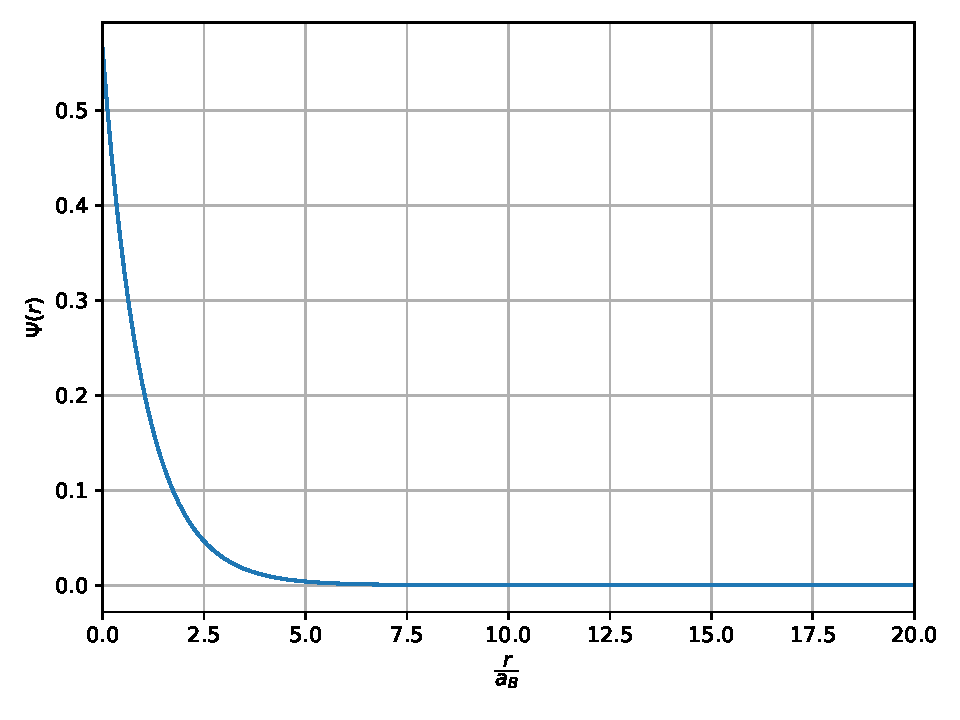
\includegraphics[width=\textwidth]{build/Graph_a.pdf} 
        \caption{Plot der Messdaten und Ausgleichsgeraden für das Impuls-Echo-Verfahren.}
        \label{fig:graph1a}
\end{figure}

\begin{figure}[H]
    \centering
    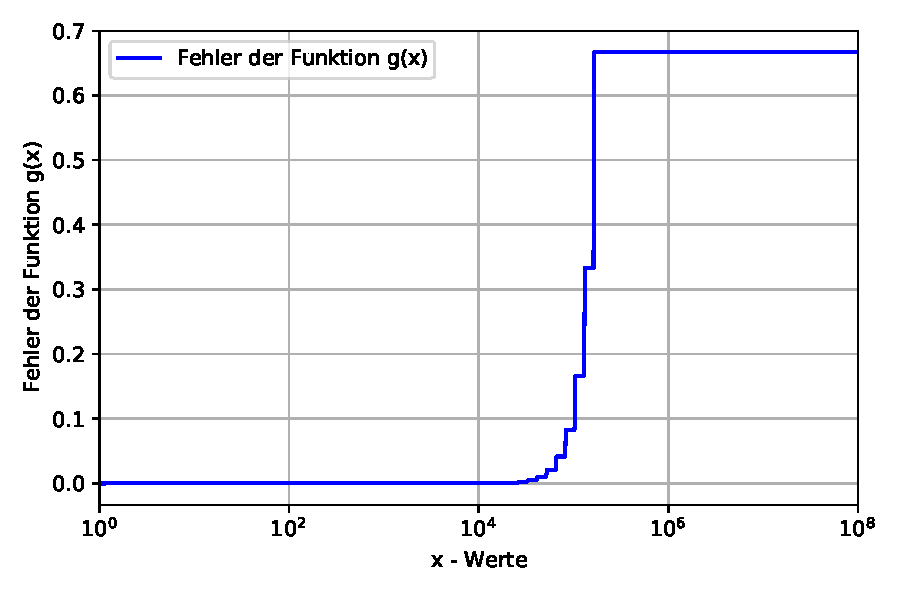
\includegraphics[width=\textwidth]{build/Graph_b.pdf} 
    \caption{Plot der Messdaten und Ausgleichsgeraden für das Durchschallungsverfahren.}
    \label{fig:graph1b}
\end{figure}

Für das Impuls-Echo-Verfahren ergeben sich die Koeffizienten dabei zu
\begin{equation*}
    c = .... \pm ... \,\unit{\frac{\meter}{\second}}
\end{equation*}
und
\begin{equation*}
    b = ... \pm ... \,\unit{\meter} \,,
\end{equation*}
für das Durchschallungsverfahren ergeben sich
\begin{equation*}
    c = .... \pm ... \,\unit{\frac{\meter}{\second}}
\end{equation*}
und
\begin{equation*}
    b = ... \pm ... \,\unit{\meter} \,.
\end{equation*} \\

Mit einem Theoriewert von
\begin{equation*}
    c_{\text{Acryl},\text{t}} = 2730 \,\unit{\frac{\meter}{\second}} 
\end{equation*}
entspricht das einer Abweichung von $... \%$ beim Impuls-Echo-Verfahren bzw. einer Abweichung von $... \%$ beim Durchschallungsverfahren.

